- Explain how data has been retrieved.

- Data provider EPEX(entsoe retrieves its data)

- Explain the ETL(Extract Transform Load) pipeline
I set up.

- Explore data in order to get useful insights for
how to tune the models to get the most of them.

- correlation between temperatures and load

- Correlation and auto correlation plots

- Split train and test dataset
Explain carefully why it is important to carry
out an out of sample test and not in sample.
In sample test involves look ahead bias because we are
fitting the model on the data we want to predict,
thus it overfits on the data considered but it does
not generalize well.


This section covers the datasets used in our experiments, attributes and features will be thoroughly described.
Next, we will explain the ETL pipeline that we set up in order to ease the workflow of our comparison studies.
Finally, in order to to bettern understand patters within the data, we carry out an exploratory data analysis.

\section{Dataset}
The chosen datasets for probabilistic load forecasting, were the data from the GEFCom 2014 competition. The data is freely hosted on Dr. Hong blog \cite{hong2016probabilistic}.
The main reason was that, these dataset are considered an a excellent test case for comparing predictive models between the EF community. Additionally, the scores of the competing models are freely available, this enables us to carry out a clean and transparent comparative study.
The GEFCom 2014 consisted of four tracks: price, load, wind power and solar power forecasting. 
The GEFCom2014 folder contains a zip file for each of the four tracks.
This thesis work is focuesed on providing forecasts for the load and price quantities.
\\
\subsection{Price track}
In the price forecasting track, the goal was to predict the electricity price for the next 24 hours of a single zone. 
The data can be found in the GEFCom2014-P\_V2 zip file alongside a set of instructions and the benchmark forecasts.
This data consisted of time series for the locational marginal price, for the zonal load and for the system load. The data covers the time interval ranging from the 1st of January 2011 to the 15th of June 2013, see figure \ref{fig:price_track_fig1}. 
Additionally, as the competition went on, the real observed data of the previous tasks were made available.
The fifteen target days ordered by task number are: 16/06/2013, 17/06/2013, 24/06/2013, 04/07/2013, 09/07/2013, 13/07/2013, 16/07/2013, 18/07/2013, 19/07/2013, 20/07/2013, 24/07/2013, 25/07/2013, 07/12/2013, 08/12/2013. 
\begin{figure}[!h]
    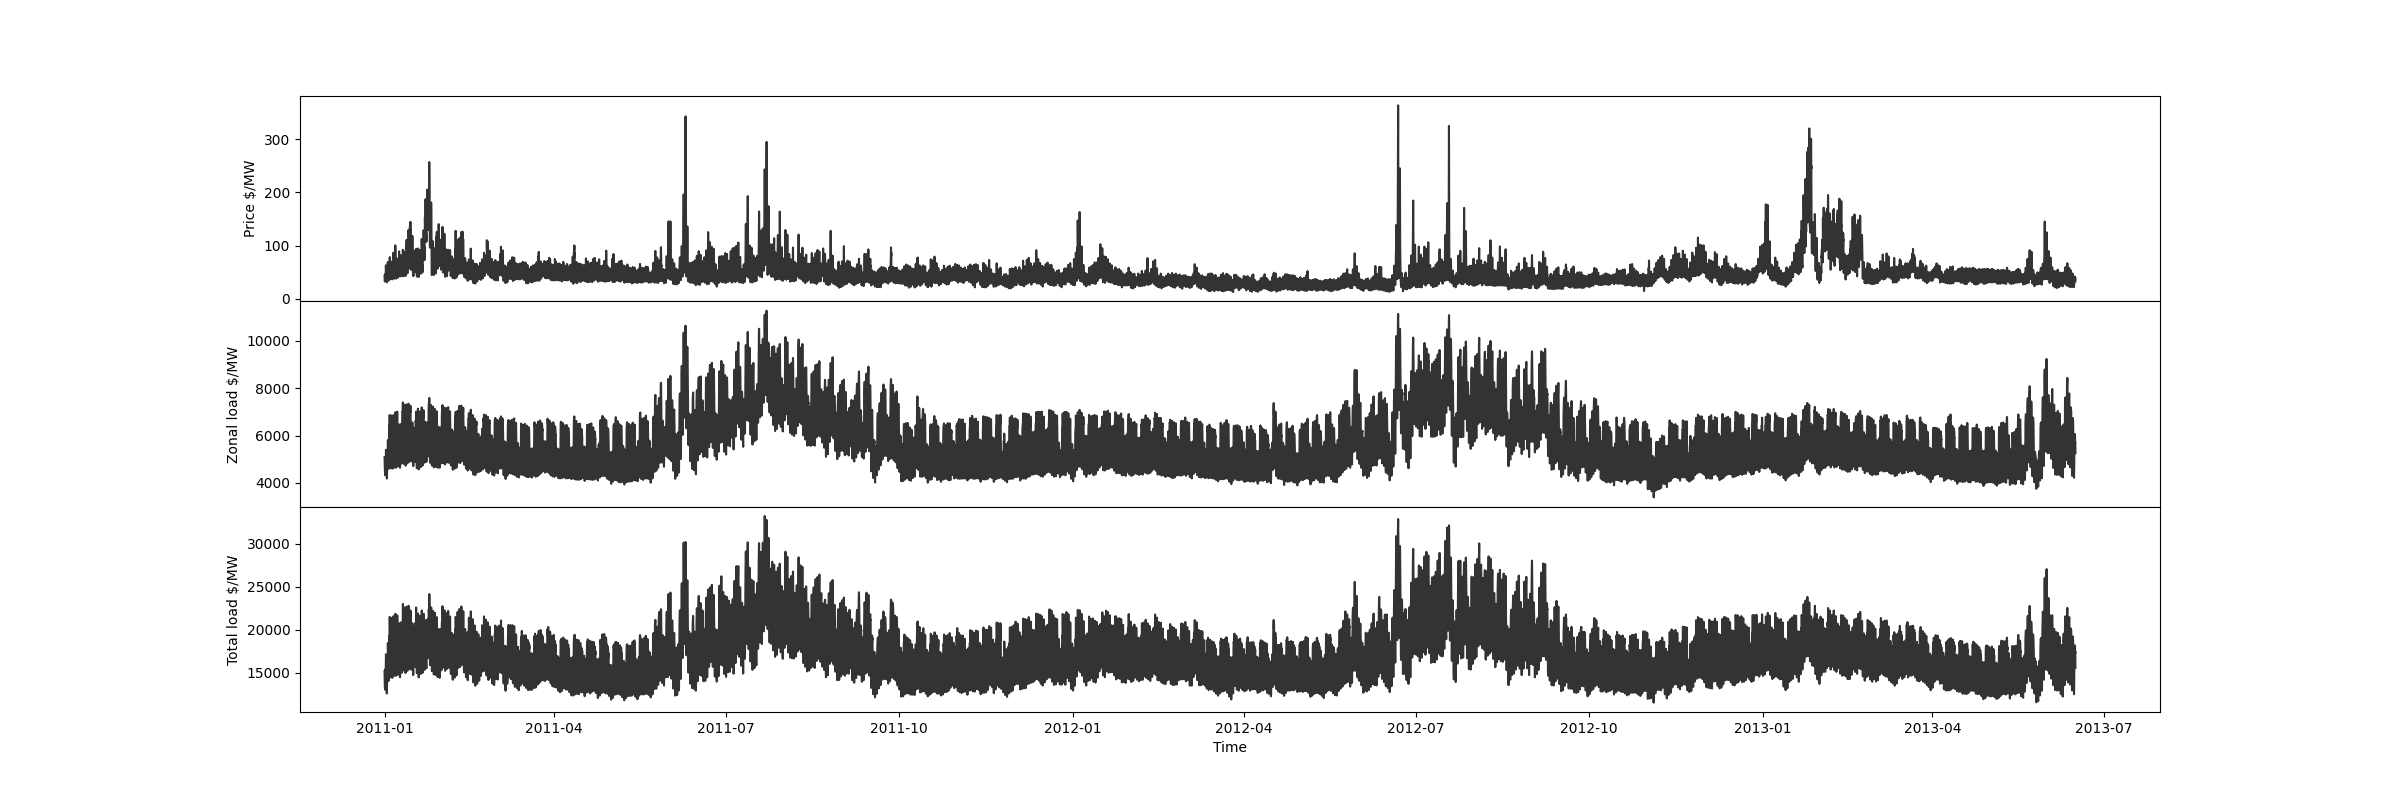
\includegraphics[width=\textwidth]{images/price_track_fig1.png}
    \caption{Price track}
    \label{fig:price_track_fig1}
\end{figure}
\subsection{Load track}
In the load track, contestant were asked to provide one month ahead hourly probabilistic forecasts on a rolling basis for 15 consecutive rounds. To get started, in the first round, organizers provided 69 months of hourly load data (from 01/01/2005 to 30/10/2010) and 117 months of hourly temperature data (from 01/01/2001 to 30/10/2010). 
As for the price track, the true observed data from the previous track were made available as the competition progressed.
\\
The data for load forecasting is contained in the GEFCom2014-L\_V2 zip file. Within this subfolder, we a txt with the competition instructions and 15 folders one for each of the consecutive tasks. For each of those we have the prediction of the competition benchmark model and the train file upon which we will fit our model.
Each data from the various task folders are shifted by one months between others.
\\
In order to compare our model performance with the winning entries of the GEFCom2014 load competition, we will refer to the Provisional\_Leaderboard\_V2 file contained also in the GEFCom2014 Data directory.
% Notice a quick premise, within this xsls file the authors opted for various scores to compare the entries performance. This choice was motivated by the need 
% to give a proportial weight to each task when averaging between them; that is in order to not penalise too much the tasks with higher point spreads. Furthermore, additional factors such as frequency of benchmark outperformance, and robustness and clarity in methodology explaination.
\\
Notice, the pinball scores for the load track are stored inside the subtab L-score-0/L-score-2 of Provisional\_Leaderboard\_V2.

\section{ETL}


\section{EDA}